\documentclass{beamer}

\setbeamertemplate{bibliography item}{\insertbiblabel}
\setlength{\parskip}{\bigskipamount}

\newcommand{\blue}[1]{\textcolor{blue}{#1}}
\newcommand{\red}[1]{\textcolor{red}{#1}}

\title{COMP390: Evolving a Sorting Algorithm with SNGP}
\author{Robin Lockyer}
\institute{University of Liverpool}
\date{03/2019}

\begin{document}
	
	\frame{\titlepage}
	
	\frame{\tableofcontents}
	
	\section{Introduction}
	
		\begin{frame}
		
			\frametitle{Project Description}
			
			Aims:
			
			\begin{itemize}
				
				\item Replicate K. E. Kinnear's work \cite{kinnear_evolving_1993} in evolving a sorting algorithm using Genetic Programming
				
				\pause
				
				\item Re-implement Kinnear's work using Single Node Genetic Programming, a variant of GP invented by Dr David Jackson\cite{jackson_new_2012}
				
				\pause
				
				\item Compare the effectiveness of the two approaches to evolving a sorting algorithm
				 
			\end{itemize}
			
			
		\end{frame}
	
		\begin{frame}
		
			\frametitle{\center{What Was Achieved?}}
			
			Successfully replicated Kinnear's work
			
			\pause
			
			Unable to evolve a sort using SNGP
			
		\end{frame}
	
	\section{Overview of Genetic Programming}
		
		\begin{frame}
		
			\frametitle{What is genetic programming?}
			
			Genetic programming is applying genetic algorithms to programmes in order
			to generate a programme that performs well in a given problem domain.
		
		\end{frame}
	
		\begin{frame}
		
			\frametitle{How Does GP Work? - 1}
			
			Programmes are encoded as a tree of primitive functions and terminals
			
			\begin{center}
				
				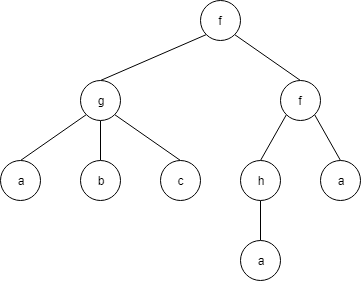
\includegraphics[scale=0.5]{resources/1_gp_example_tree}
				
				This tree encodes the programme f( g( a, b, c ), f( h( a ), a ) ), where f, g, and h are functions and a, b, and c are terminals.
				
			\end{center}
			
			
		
		\end{frame}
	
		\begin{frame}
			
			\frametitle{How does GP Work? - 2}
			
			\begin{center}
				
				An initial population of random programmes is created
				
				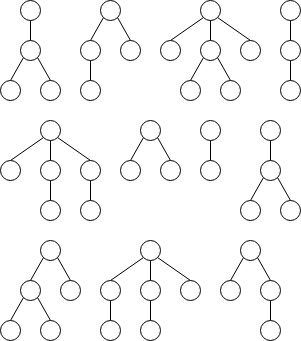
\includegraphics[scale=0.4]{resources/2_gp_example_population}
				
			\end{center}
			
		\end{frame}
	
		\begin{frame}
		
			\frametitle{How Does GP Work? - 2}
			
			\begin{center}
				
				An initial population of random programmes is created
				
				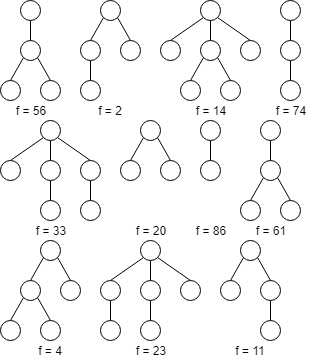
\includegraphics[scale=0.4]{resources/3_gp_example_fitness}
				
				Each member of the population is executed, evaluated, and given a fitness score
				
			\end{center}
			
		\end{frame}
	
		\begin{frame}
		
			\frametitle{How Does GP Work? - 3}
			
			\begin{center}
			
				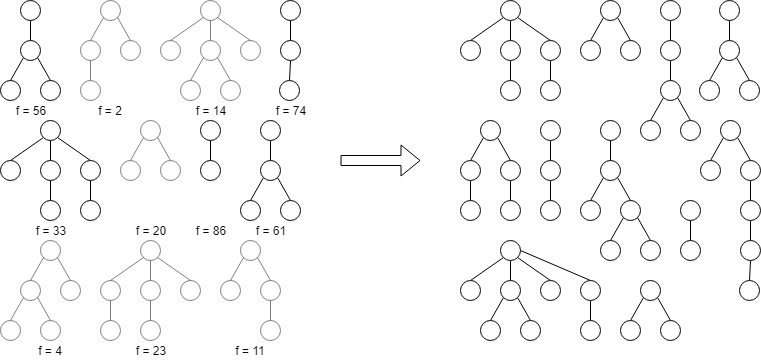
\includegraphics[scale=0.4]{resources/4_gp_example_selection}
				
				A new population is created by selecting some of the most fit members of the initial population and performing genetic operations on them to create new programmes
				
			\end{center}
		
		\end{frame}
	
		\begin{frame}
			
			\frametitle{How Does GP Work? - 4}
			
			There are three main genetic operators:
			
			\medskip
			\pause
			
			\begin{columns}[T]
				
				\begin{column}{0.2\textwidth}
					
					\blue{Reproduction}
					
					\medskip
					
					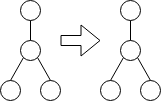
\includegraphics[scale=0.35]{resources/5_reproduction}
					
					\begin{small}
						A programme is copied over to the new population without any changes
					\end{small}
				
				\end{column}
			
				\pause
			
				\begin{column}{0.4\textwidth}
					
					\blue{Crossover}
					
					\medskip
					
					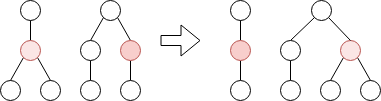
\includegraphics[scale=0.35]{resources/6_crossover}
					\begin{small}
						A random node is selected in each of the chosen programmes. The subtrees rooted at the selected nodes are swapped.
					\end{small}
			
				\end{column}
			
				\pause
			
				\begin{column}{0.3\textwidth}
					
					\blue{Mutation}
					
					\medskip
					
					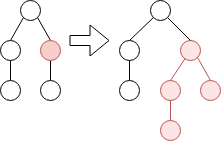
\includegraphics[scale=0.35]{resources/7_mutation}
					
					\begin{small}
						A random node is selected in the chosen programme. A new, random subtree is generated to replace the subtree rooted at the selected node.
					\end{small}
				\end{column}
				
			\end{columns}
			
		\end{frame}
	
		\begin{frame}
		
			\frametitle{How Does GP Work? - 5}
			
			This process is repeated until a programme with high enough fitness is generated
		
		\end{frame}
	
	
	\section{Overview of Single Node Genetic Programming}

		\begin{frame}
			
			\large{\blue{What is SNGP?}}
			
			\medskip
			
			\pause
			
			\begin{itemize}
				\item SNGP is a variation of GP that organises the whole population into a single interlinked graph
				
				\pause
				
				\item The subtree rooted at each node in the graph is considered to be an individual programme
				
				\pause
				
				\item The graph is structured in such a way that a form of dynamic programming can be used to increase the efficiency of evaluating the population
			\end{itemize}
			
		\end{frame}
	
		\begin{frame}
		
			\frametitle{SNGP Population - 1}
			
			\center{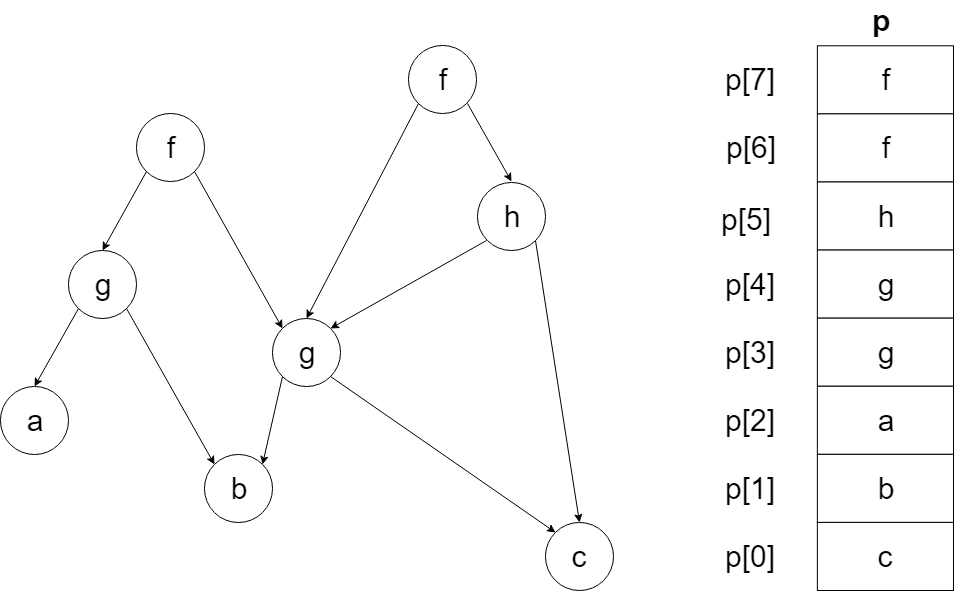
\includegraphics[scale=0.7]{resources/8_sngp_graph}}
					
			\begin{itemize}
				\pause
				\item Graph nodes are stored in an array
				\pause
				\item Terminals are stored in the lowest elements
				\pause
				\item Remaining elements store a random function
				\pause
				\item Each function's operands are chosen from elements with a smaller index
			\end{itemize}
				
		
		\end{frame}
	
		\begin{frame}
			\frametitle{SNGP Population - 2}
			
			\begin{columns}
				
				\begin{column}{0.4\textwidth}
					
					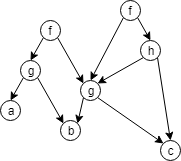
\includegraphics[scale=0.7]{resources/9_sngp_graph_no_array}
					
				\end{column}
			
				\begin{column}{0.6\textwidth}
					
					This graph contains the following programmes:
					
					\begin{itemize}
						\item a
						\item b
						\item c
						\item g( b, c )
						\item g( a, b )
						\item h( g( b, c ), c )
						\item f( g( a, b ), g( b, c ) )
						\item f( g( b, c ), h( g( b, c ), c ) )
					\end{itemize}
					
				\end{column}
				
			\end{columns}
			
		\end{frame}
	
		\begin{frame}
			\frametitle{SNGP Operators}
			
			SNGP has only one genetic operator:
			
			\begin{center}
				
				\blue{Successor Mutate}
				
				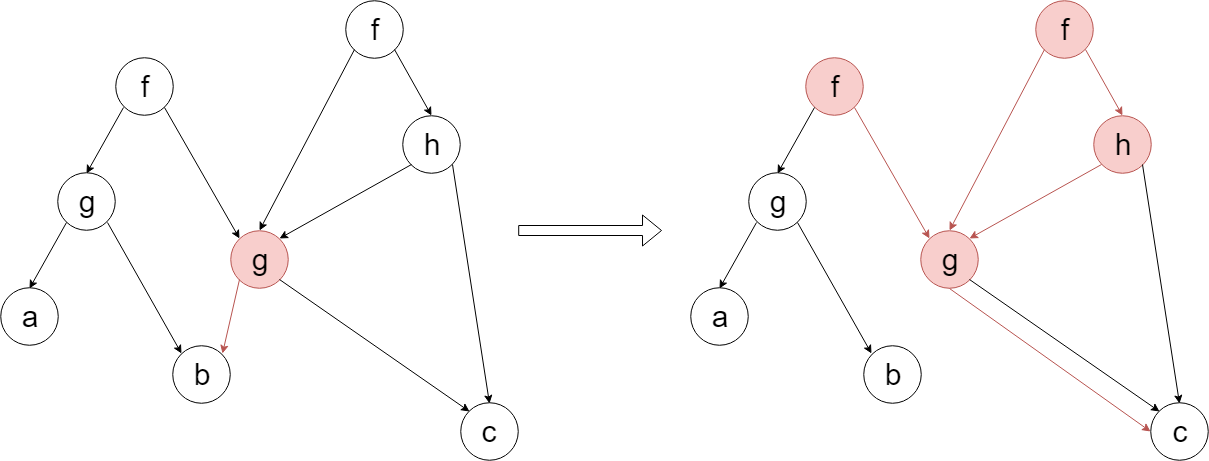
\includegraphics[scale=0.5]{resources/10_successor_mutate}
				
				A random node is chosen and one of its operands is randomly changed. This causes the programmes represented by both the chosen node and all of its predecessors to be altered.
				
			\end{center}
			
		\end{frame}
	
		\begin{frame}
			\frametitle{Calculating Fitness - 1}
			
			\begin{center}
			
				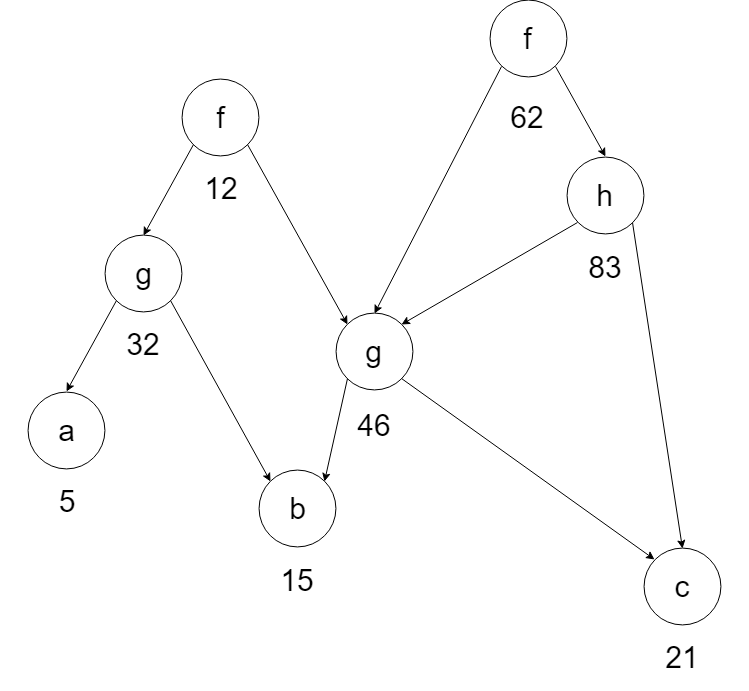
\includegraphics[scale=0.5]{resources/11_sngp_fitness}
				
				
			\end{center}
			
			Each individual is executed, evaluated and given a fitness,and then the whole population is given a fitness as a whole. 
			
			If a change to the population does not improve this overall fitness, the change is reverted and a different node is selected for the genetic operator.

		\end{frame}
	
		\begin{frame}
			\frametitle{Calculating Fitness - 2}
			
			\begin{center}
				
				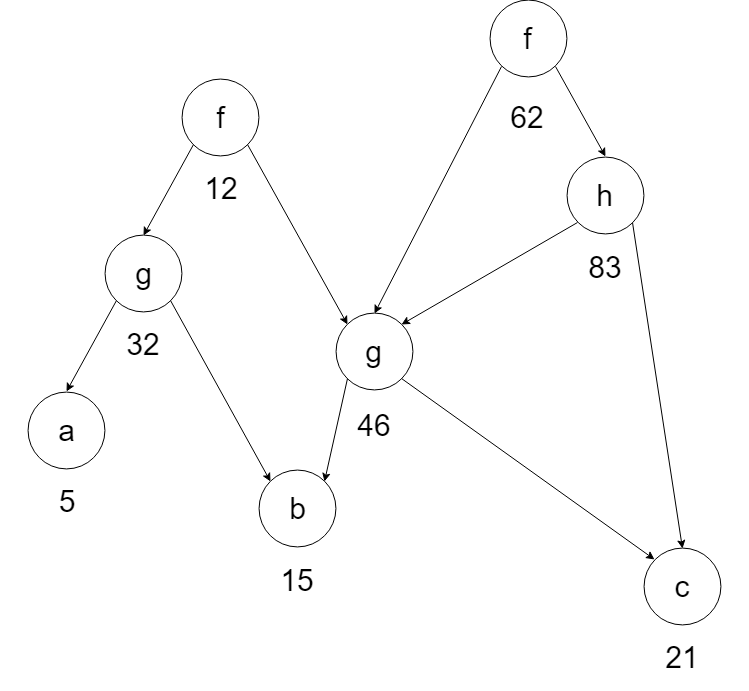
\includegraphics[scale=0.5]{resources/11_sngp_fitness}
				
				
			\end{center}
			
			There are two methods of giving the population a fitness:
			
			\begin{itemize}
				\item SNGP/A: The fitness of the population is the \blue{average} of each individual fitness. In the diagram above this fitness is 34.5.
				\item SNGP/B: The fitness of the population is the fitness of \blue{best} individual. In the diagram above this fitness is 83.
			\end{itemize}
				
	
		\end{frame}
	
		\begin{frame}
		
			\frametitle{Benefits}
					
			\begin{itemize}
				
				\item When using pure functions the graph structure allows for dynamic programming by re-using the results from executing subtrees, making evaluation more efficient.
				\item A single application of successor mutate can modify many individuals at once
				\item When re-evaluating after successor mutate, results from the previous generation can be used to speed up the evaluation of the graph.
				\item SNGP tends to find solutions more often than SNGP \cite{jackson_new_2012, jackson_single_2012}.
				\item SNGP allows for a single programme to re-use code, resulting in smaller programmes \cite{jackson_new_2012}.
				
			\end{itemize}
			
			\pause
			
			However:
			
			When using functions with side effects SNGP cannot make use of dynamic programming as the result of executing subtrees changes depending on what was executed before.

		
		\end{frame}
		
	\section{Reproducing Kinnear's Results}
	
		\begin{frame}
		
			\frametitle{Reproducing Kinnear's Results}
			
			I was successful in reproducing Kinnear's results.
			
			\pause
			
			Following the method set out in \cite{kinnear_generality_1993} and \cite{kinnear_evolving_1993} immediately lead to evolving a sort.
			
			\pause
			
			With a population of 1000 Kinnear's method would consistently find a solution within 50 generations.
			
		\end{frame}
	
		\begin{frame}
		
			\frametitle{Implementation Details}
			
			Implementation based on example code provided by Dr Jackson from his past experiments with GP, and also on an implementation of the TinyGP system found in the book "A Field Guide to Genetic Programming" \cite{poli_field_2008}.
			
			Some changes from Dr Jackson's code has to be made to follow Kinnear's method.
		
		\end{frame}
	
		\begin{frame}
			
			\frametitle{Implementing Primitives}
			
			The primitives used were the same nine described by Kinnear in \cite{kinnear_evolving_1993}, although I renamed some to make their function more clear.
			
			\begin{columns}[T]
				
				\begin{column}{0.5\textwidth}
					
					\begin{itemize}
						\item INDEX
						\item LENGTH
						\item ITERATE(start, end, function)
						\item SWAP(x, y)
						\item SMALLEST(x, y)
					\end{itemize}
					
				\end{column}
			
				\begin{column}{0.5\textwidth}
					
					\begin{itemize}
					\item LARGEST(x, y)
					\item SUBTRACT(x, y)
					\item INCREMENT(x)
					\item DECREMENT(x)
					\end{itemize}
					
				\end{column}
				
			\end{columns}
	
		\end{frame}
	
		\begin{frame}
		
			\frametitle{Fitness Function}
			
			Kinnear's fitness function as described in \cite{kinnear_generality_1993} is as follows:
			
			
				\begin{columns}[T]
					
					\begin{column}{0.5\textwidth}
						
						\begin{tiny}
							
						$$fitness(prog) = \frac{adjusted(prog)}{\sum_{p\in population}^{}adjusted(p)}$$
						
						$$adjusted(prog) = \frac{1}{1 + raw(prog)}$$
						
						$$raw(prog) = praw(prog) - \min_{p\in population} praw(p)$$
						
						\end{tiny}
					
					
					\end{column}
					
					
					\begin{column}{0.5\textwidth}
						
						\begin{tiny}
						
						$$praw(prog) = \left(\sum_{t = 1}^{Number Of Tests}res(t)\right) \cdot of + size(prog) \cdot sf$$
						
						$$res(t) = rdis(t) + pdis(t)$$
						
						$$pdis(t) = max(rdis(t) - idis(t), 0) \cdot 100$$
						
						\end{tiny}
					\end{column}
				\end{columns}
			
			Where rdis(t) is the remaining number of inversions in a test array t after running a member of the population, idis(t) is the initial number of inversions in a test array t, and of and sf are constant weights used to adjust the resulting fitness.
		
		\end{frame}
	
	\section{Attempting SNGP}
	
	\section{Conclusion}
	
	\section{Bibliography}
	
		\begin{frame}[allowframebreaks] 
			\frametitle{Bibliography}
			\bibliographystyle{acm}
			\bibliography{library}
		\end{frame}
		
\end{document}